\documentclass[12pt,letterpaper,final]{article}

\usepackage{Sweave}
\usepackage{graphicx}
\usepackage{natbib}
\usepackage{hyperref}
\usepackage{caption}
\usepackage{rotating}
\usepackage{verbatim}
\usepackage{textcomp}
\usepackage{wasysym}

\setlength{\oddsidemargin}{0in}
\setlength{\textwidth}{6.15in}
%\setlength{\topmargin}{0.5in}
\setlength{\textheight}{22cm}
\setlength{\headheight}{0in}
\setlength{\headsep}{0in}
\setlength{\parskip}{5pt plus 2pt minus 3pt}

\def\thefootnote{\fnsymbol{footnote}}
\setcounter{footnote}{1}

\renewcommand{\baselinestretch}{1.2}
\renewcommand{\labelenumi}{(\roman{enumi})}

\renewcommand{\topfraction}{1.0}
\renewcommand{\bottomfraction}{1.0}
\renewcommand{\textfraction}{0.0}
\renewcommand{\floatpagefraction}{1.0}

\newtheorem{definition}{Definition}
\newtheorem{theorem}{Theorem}
\newtheorem{lemma}[theorem]{Lemma}
\newtheorem{claim}[theorem]{Claim}
\newtheorem{fact}[theorem]{Fact}

% to get nice proofs ...
\newcommand{\qedsymb}{\mbox{ }~\hfill~{\rule{2mm}{2mm}}}
\newenvironment{proof}{\begin{trivlist}
\item[\hspace{\labelsep}{\bf\noindent Proof: }]
}{\qedsymb\end{trivlist}}


\newfont{\msymb}{cmsy10 scaled 1000}

\def\nullset{\mbox{\O}}
\def\R{{I\!\!R}}
\def\C{{I\!\!\!\!C}}
\def\N{{I\!\!N}}

\def\P{\mbox{\msymb P}}


%\parskip 0.1in
\pagenumbering{arabic}    %  Start using 1,2,... as page numbers.
\pagestyle{plain}         %  Page numbers in middle bottom of page.
%\setcounter{page}{80}  % XXXXXXXXXXXXXXXXX
%\setcounter{theorem}{5} % XXXXXXXXXXXXXXXXX
%\setcounter{definition}{10} % XXXXXXXXXXXXXXXXX

\parindent 0in


\begin{document}

\Sconcordance{concordance:rnw_example.tex:rnw_example.Rnw:%
1 118 1 1 2 1 0 3 1 3 0 1 2 7 1 1 2 1 0 1 3 5 0 1 2 9 1 1 9 12 0 1 2 19 %
1 1 2 5 0 1 2 6 1 1 10 13 0 1 2 22 1 1 3 6 0 1 2 6 1 1 9 12 0 1 2 16 1 %
1 2 5 0 1 2 6 1 1 9 12 0 1 2 19 1 1 3 6 0 1 2 10 1 1 9 12 0 1 2 16 1 1 %
2 5 0 1 2 6 1 1 7 10 0 1 2 44 1 1 3 2 0 1 4 1 0 1 2 4 0 1 2 17 1 1 2 1 %
0 1 3 6 0 1 3 8 0 1 2 27 1 1 3 2 0 2 2 1 4 3 0 1 5 4 0 1 4 3 0 1 7 10 0 %
1 2 21 1 1 9 12 0 1 2 23 1 1 2 1 0 1 1 2 3 5 0 1 2 60 1}


\begin{table}\centering
\begin{tabular*}{6.15in}{@{\extracolsep{\fill}}|llr|} \hline
RNW Example File & \hspace*{0.5 in} & Fall 2019 \\
 & & \\
\multicolumn{3}{|c|}{
{\bf Name:} Michael Huber} \\
 & & \\
\multicolumn{3}{|c|}{
{\bf Submission Date:} 10/17/2019} \\
 & & \\
\multicolumn{3}{|c|}{
Data Visualization Document (10/02/2019)} \\
 & & \\
\multicolumn{3}{|c|}{
45 Points --- Due Friday 10/18/2019 (via Canvas by 11:59pm)} \\
\hline
\end{tabular*}
\end{table}


~ \newpage

\begin{enumerate}

\item (35 Points)
In this question, you have to work with the {\it faithful} data set from {\bf datasets} in baseR. 
Be aware that different versions of this data set exist. Do not use any of
the other versions or your results will differ slightly as different versions
of the data set
could be considered to be different samples from the same underlying geological process.

The help page for the {\it faithful} data set indicates:
\begin{verbatim}
Old Faithful Geyser Data

Description
Waiting time between eruptions and the duration of the eruption for 
the Old Faithful geyser in Yellowstone National Park, Wyoming, USA.

Usage
faithful

Format
A data frame with 272 observations on 2 variables.
[,1]	 eruptions	 numeric	 Eruption time in mins
[,2]	 waiting	 numeric	 Waiting time to next eruption (in mins)
\end{verbatim}

\begin{enumerate}
\item (1 Point) Load all required R packages to answer this question. Show your R code.

\begin{Schunk}
\begin{Sinput}
> library(ggplot2)
> library(gridExtra)
> library(MASS)
> library(vioplot)
\end{Sinput}
\end{Schunk}





\item (1 Point) Draw a basic histogram for {\it eruptions} using ggplot2.
Include your R code and the resulting graph.

\begin{Schunk}
\begin{Sinput}
> data <- faithful
> ggplot(data, aes(x = eruptions)) + 
+   geom_histogram()
\end{Sinput}
\end{Schunk}
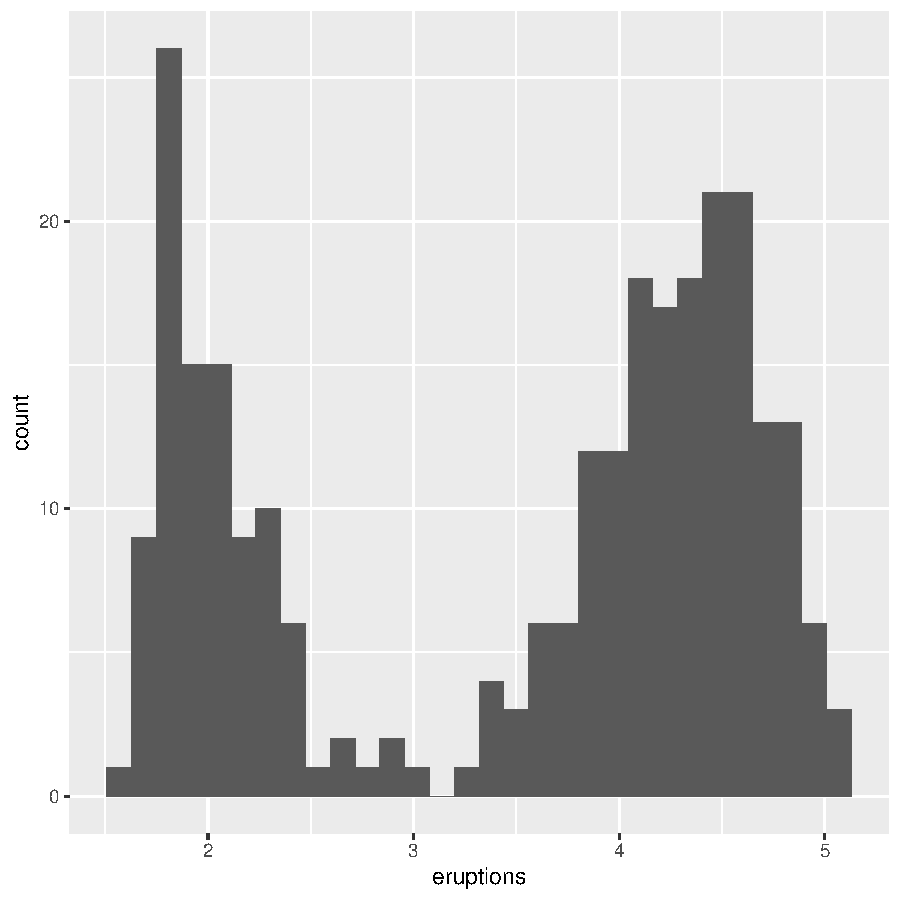
\includegraphics{rnw_example-002}





\item (3 Points) Further improve your histogram from (b). You may want to adjust the binwidth,
starting points of the intervals, labels, title, etc. Clearly indicate which changes
you made and why you made these changes. Include your final graph and the R code
for the final graph. No need to include any intermediate graphs and the R code for those.

\begin{Schunk}
\begin{Sinput}
> ggplot(data, aes(x = eruptions)) + 
+   scale_x_continuous(breaks = seq(0, 6, .5)) +
+   scale_y_continuous(breaks = seq(0, 100, 10)) +
+   geom_histogram(binwidth = .5, fill = "light blue", color = "black") +
+   xlab("Eruption Time in Minutes") +
+   ylab("Count of Eruptions") +
+   ggtitle("Old Faithful Eruption Data Histogram") +
+   theme(plot.title = element_text(hjust = 0.5))
\end{Sinput}
\end{Schunk}
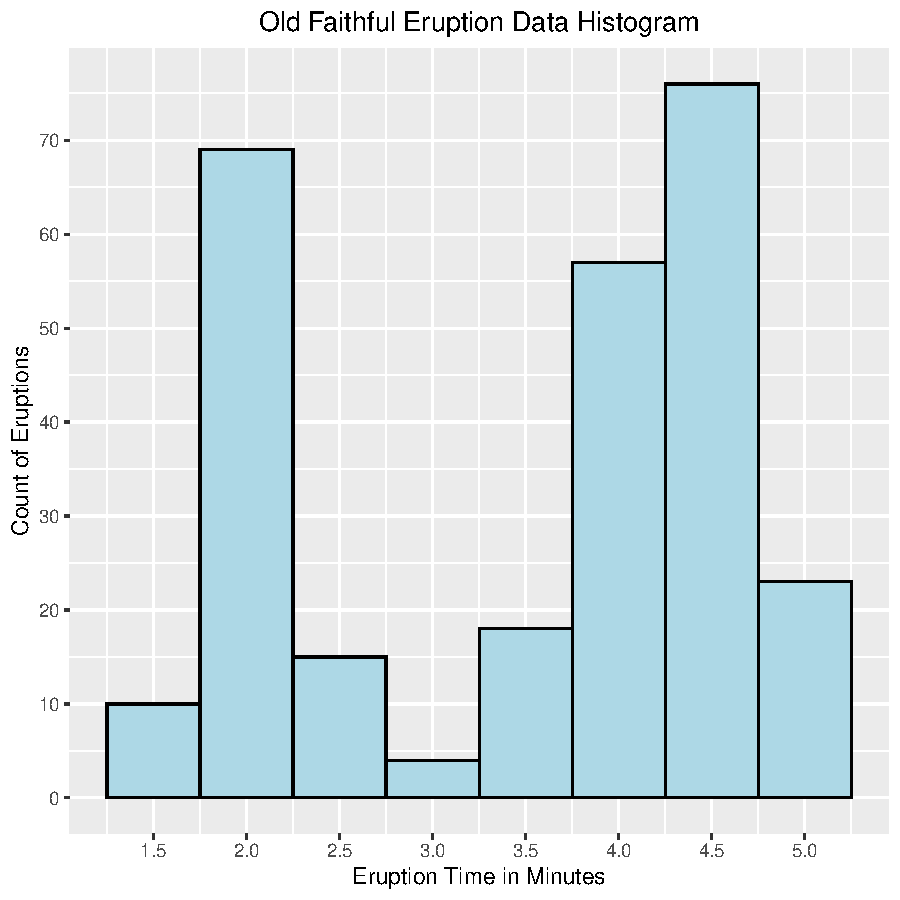
\includegraphics{rnw_example-003}

\underline{Answer:} Changes made:
\begin{itemize}
\item Added scale x continuous so that the data would all fit on the x axis and define line breaks
\item Added scale y coninuous To be able to define the line breaks on the y axis
\item Added xlab to label that the x axis show the duration of the eruption in minutes
\item Added ylab to label the number of eruptions that were occuring for each time block
\item Added binwidth of .5 to break each bin into 30 second increments.
\item Added fill = "light blue" to add some color to contrast with the background
\item Added color = "black" to define the separation between different bars
\item Added ggtitle() to label that this was Old Faithfuls eruption Data
\item Added theme(plot.title = element text(hjust = 0.5)) to center the title over the graph
\end{itemize}





\item (1 Point) Repeat (b) from above, now using the {\it hist} function from baseR.

\begin{Schunk}
\begin{Sinput}
> hist(faithful$eruptions)
\end{Sinput}
\end{Schunk}
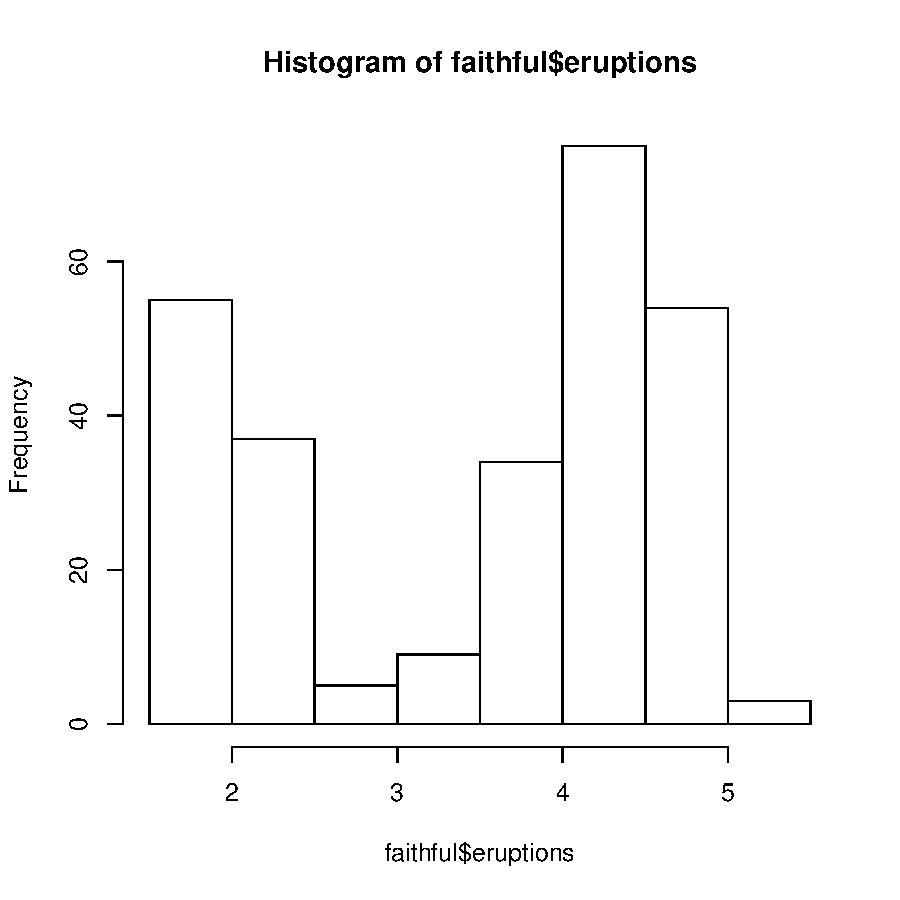
\includegraphics{rnw_example-004}





\item (3 Points) Repeat (c) from above, now using the {\it hist} function from baseR.

\begin{Schunk}
\begin{Sinput}
> hist(faithful$eruptions,
+      breaks = seq(1, 6, .5),
+      xlab = "Eruption Time in Minutes",
+      ylab = "Count of Eruptions",
+      main = "Old Faithful Eruption Data Histogram",
+      col = "light blue",
+      las = 1,
+      ylim = c(0, 100),
+      xlim = c(1, 6))
\end{Sinput}
\end{Schunk}
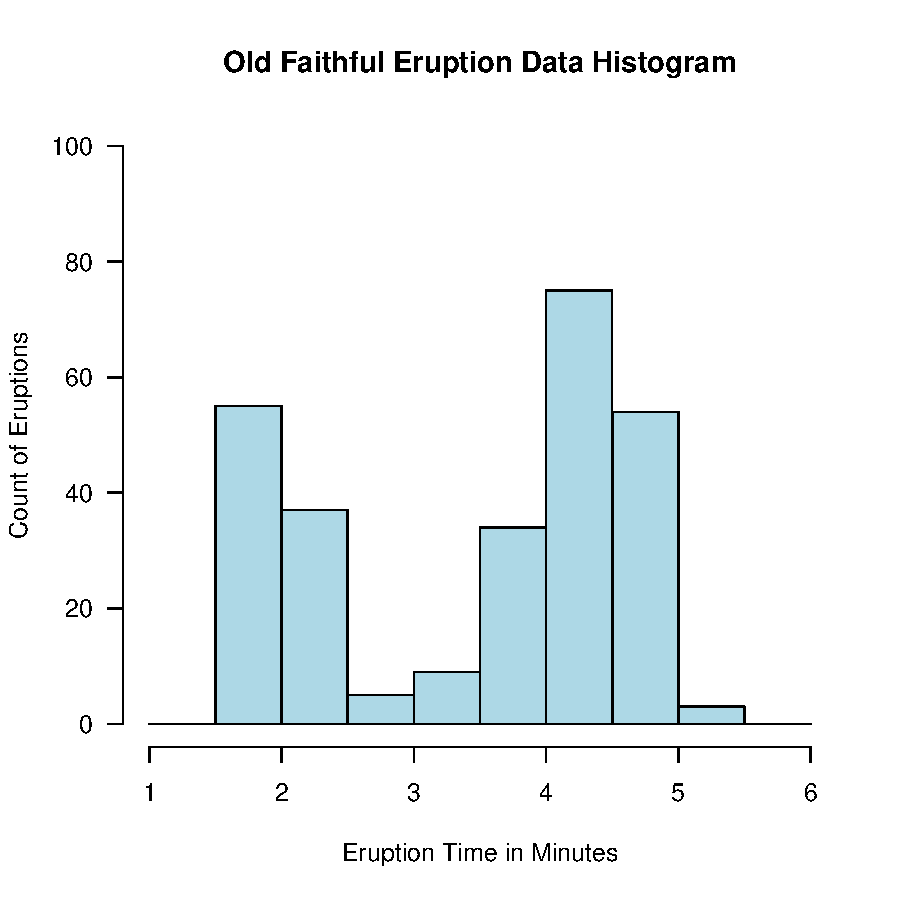
\includegraphics{rnw_example-005}

\underline{Answer:} Changes made:
\begin{itemize}
\item Added breaks to the hist function which adjusted the groups that the bars were broken in to. It also sets the width
of the x-axis.
\item Added xlab and ylab to label what was being displayed on each axis.
\item Added main to add a title to the graph
\item Added col with light blue to add a light blue color to the bins.
\item Added las = 1 which flips the numbers on the y axis from being on their sides to standing upright.
\item Added ylim so that the y axis would be numbered to the top of the graph.
\end{itemize}

\underline{References Used to Solve this Problem:}
\begin{itemize}
\item https://www.datacamp.com/community/tutorials/make-histogram-basic-r
\end{itemize}





\item (1 Point) Repeat (b) from above, now for {\it waiting}.

\begin{Schunk}
\begin{Sinput}
> ggplot(faithful, aes(x = waiting)) + 
+   geom_histogram()
\end{Sinput}
\end{Schunk}
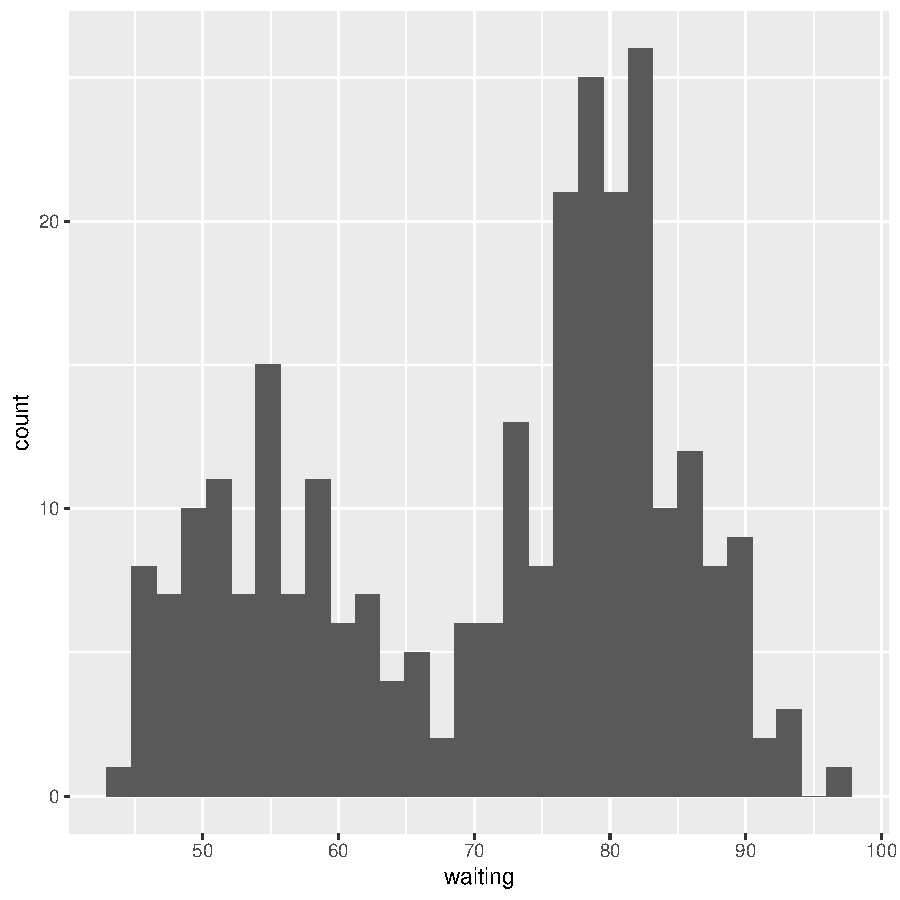
\includegraphics{rnw_example-006}





\item (3 Points) Repeat (c) from above, now for {\it waiting}.

\begin{Schunk}
\begin{Sinput}
> ggplot(faithful, aes(x = waiting)) + 
+   scale_x_continuous(breaks = seq(0, 100, 10)) +
+   scale_y_continuous(breaks = seq(0, 70, 10)) +
+   geom_histogram(binwidth = 5, fill = "light blue", color = "black") +
+   xlab("Waiting Time Between Eruptions in Minutes") +
+   ylab("Count of Waiting Times") +
+   ggtitle("Old Faithful Waiting Time Between Eruptions") +
+   theme(plot.title = element_text(hjust = 0.5))
\end{Sinput}
\end{Schunk}
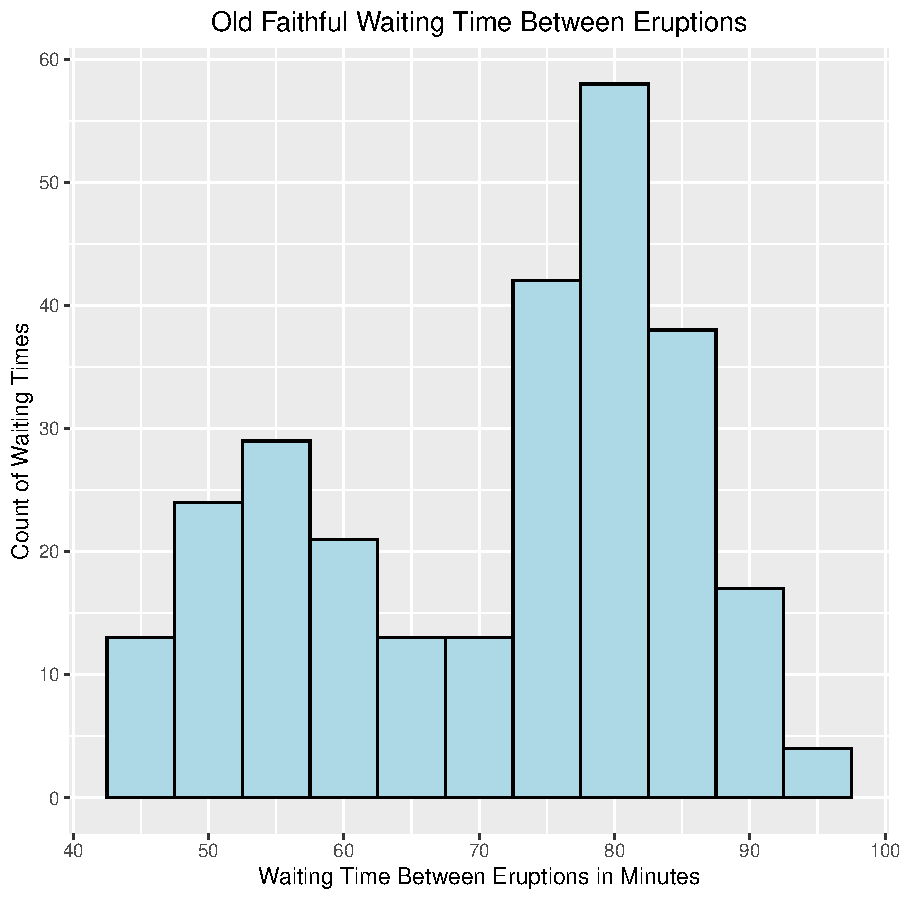
\includegraphics{rnw_example-007}

\underline{Answer:}
\begin{itemize}
\item Added scale x continuos to set the x axis number breaks to intervals of 10.
\item Added scale y continuous to set the y axis number breaks to intervals of 10.
\item Added binwidth = 5 so that each bin represents 5 minute segments.
\item Added a fill = light blue and color = black so that it was easier to distinguish between each bin.
\item Added a xlab and ylab to describe what each axis was measuring.
\item Added ggtitle to give a title to the graph, along with the plot.title to center it over the graph.
\end{itemize}





\item (1 Point) Repeat (d) from above, now for {\it waiting}.

\begin{Schunk}
\begin{Sinput}
> hist(faithful$waiting)
\end{Sinput}
\end{Schunk}
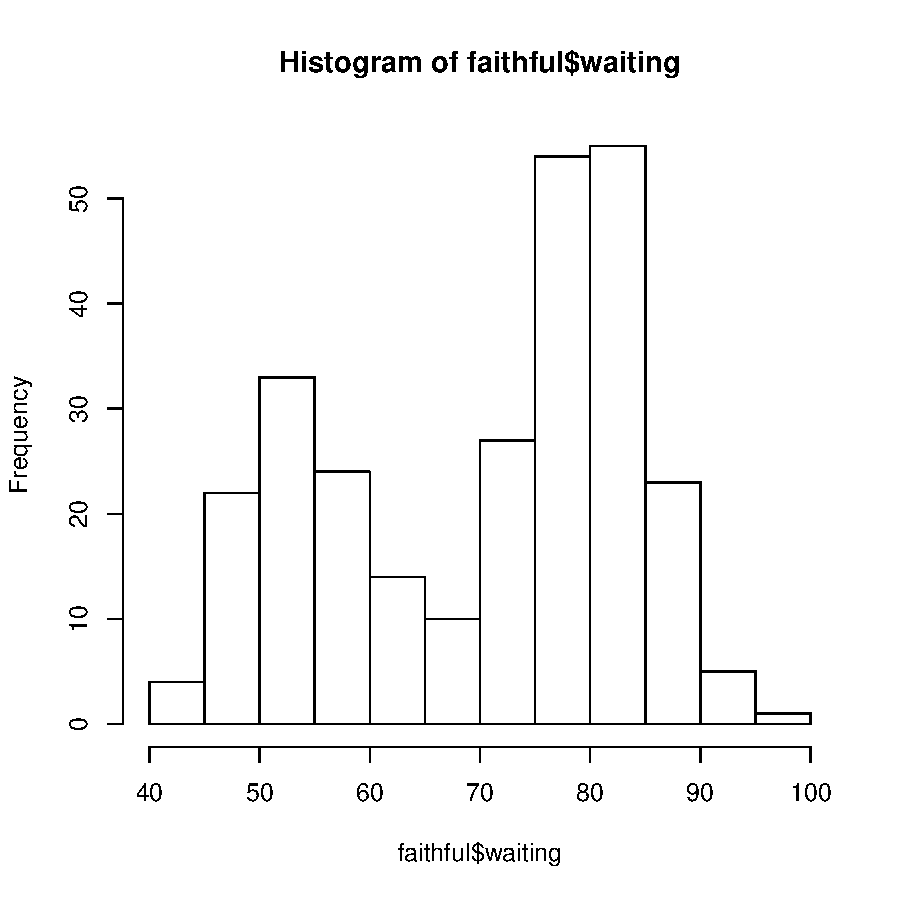
\includegraphics{rnw_example-008}





\item (3 Points) Repeat (e) from above, now for {\it waiting}.

\begin{Schunk}
\begin{Sinput}
> hist(faithful$waiting,
+      breaks = seq(40, 100, by = 5),
+      xlab = "Waiting Time Between Eruptions in Minutes",
+      ylab = "Old Faithful Waiting Time Between Eruptions",
+      main = "Wait Time Between Eruptions Histogram",
+      col = "light blue",
+      las = 1,
+      ylim = c(0, 70))
\end{Sinput}
\end{Schunk}
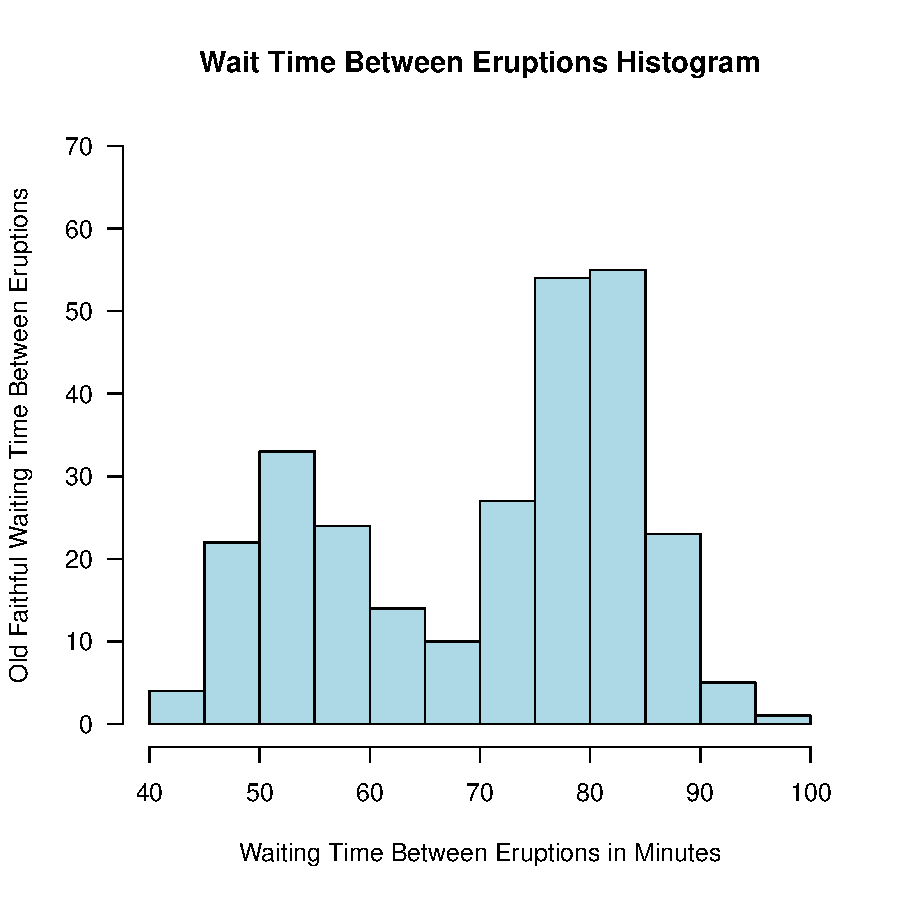
\includegraphics{rnw_example-009}

\underline{Answer:}
\begin{itemize}
\item Added breaks into the his function to cover the range of waiting times and give a binwidth of 5 which means
each bin is equal to 5 minutes.
\item Added xlab and ylab to label each of the axis to tell the reader what they measure.
\item Added main to give the graph a title to let the reader know the overall purpose of the graph.
\item Added col = light blue so that the bars of the graph would stand out against the page.
\item Added las = 1 so that the numbers of the y axis would stand upright.
\item Added ylim to define how high the y axis will go.
\end{itemize}





\item (1 Point) Draw a basic scatterplot of the two variables using ggplot2. Assume that {\it eruptions}
is the explanatory variable.
Include your R code and the resulting graph.

\begin{Schunk}
\begin{Sinput}
> ggplot(faithful, aes(x = eruptions, y = waiting)) +
+   geom_point()
\end{Sinput}
\end{Schunk}
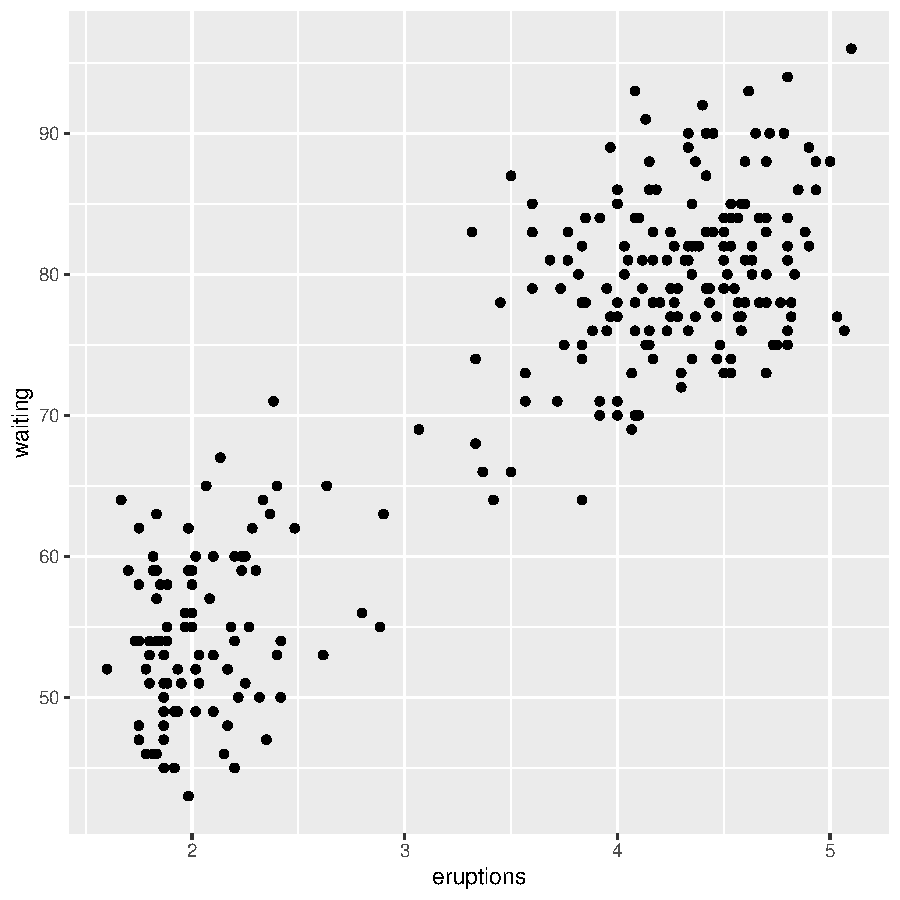
\includegraphics{rnw_example-010}





\item (3 Points) Further improve your scatterplot from (j). 
You may want to adjust the range of the axes, labels, etc. 
Clearly indicate which changes
you made and why you made these changes. Include your final graph and the R code
for the final graph. No need to include any intermediate graphs and the R code for those.

\begin{Schunk}
\begin{Sinput}
> ggplot(faithful, aes(x = eruptions, y = waiting)) +
+   scale_x_continuous(breaks = seq(0, 6, .25)) +
+   scale_y_continuous(breaks = seq(40, 100, 5)) +
+   geom_point(color="blue") +
+   xlab("Eruption Time in Minutes") +
+   ylab("Wait Time Between Eruptions in Minutes") +
+   ggtitle("Old Faithful Eruption & Wait Time Scatter Plot") +
+   theme(plot.title = element_text(hjust = 0.5))
\end{Sinput}
\end{Schunk}
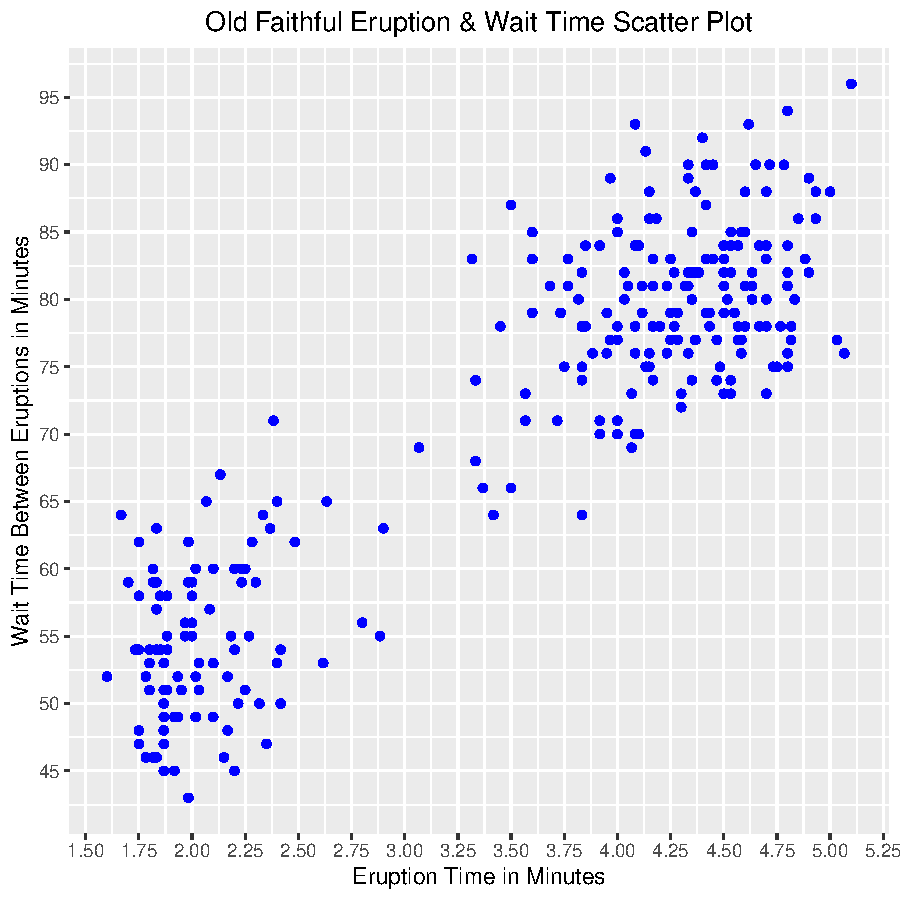
\includegraphics{rnw_example-011}

\underline{Answer:}
\begin{itemize}
\item Added scale x continuous to be able to more easily identify what is the time for the eruption values.
\item Added scale y continuouse to be able to more easily identify the value for the waiting variable.
\item Added xlab and ylab labels to both axes to explain what each axis is showing on the graph.
\item Added ggtitle to let the reader know what the graph was displaying.
\item Added theme plot.title to center the title over the graph.
\item Added color = blue to contrast with the background of the graph.
\end{itemize}





\item (1 Point) Repeat (j) from above, now using the {\it plot} function from baseR.

\begin{Schunk}
\begin{Sinput}
> plot(faithful$eruptions, faithful$waiting)
\end{Sinput}
\end{Schunk}
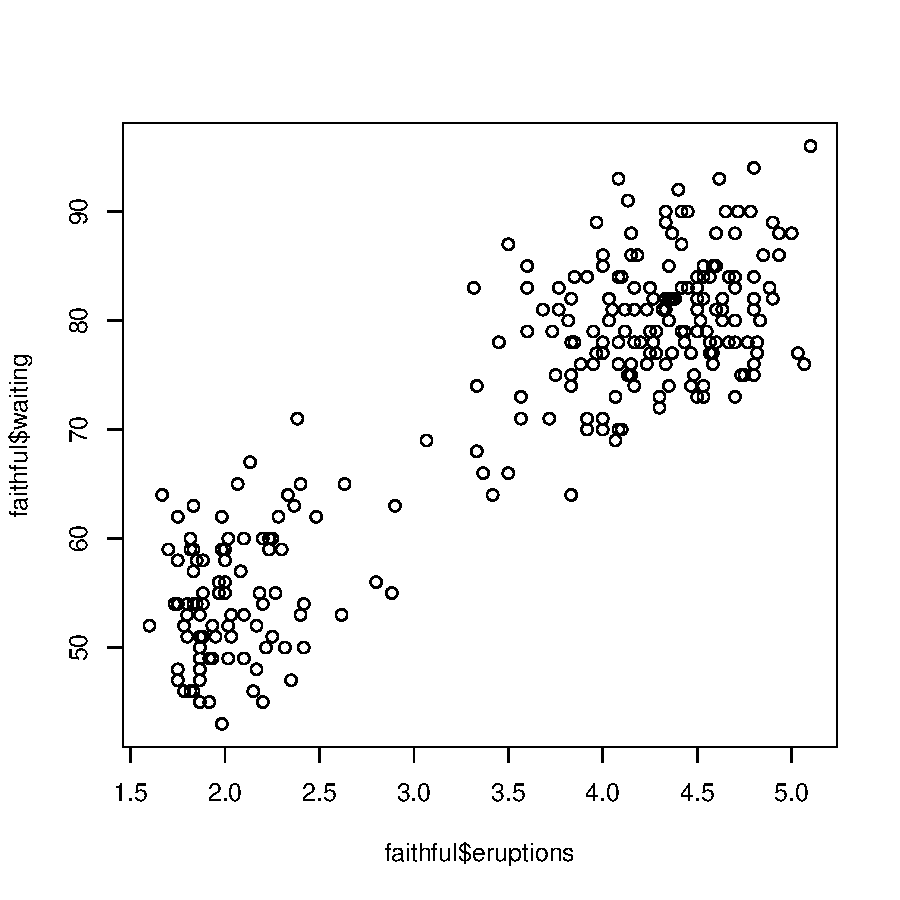
\includegraphics{rnw_example-012}





\item (3 Points) Repeat (k) from above, now using the {\it plot} function from baseR.

\begin{Schunk}
\begin{Sinput}
> plot(faithful$eruptions, faithful$waiting,
+      xlab = "Eruption Time in Minutes",
+      ylab = "Wait Time Between Eruptions in Minutes",
+      main = "Old Faithful Eruption & Wait Time Scatter Plot",
+      col = "blue",
+      pch = 16)
\end{Sinput}
\end{Schunk}
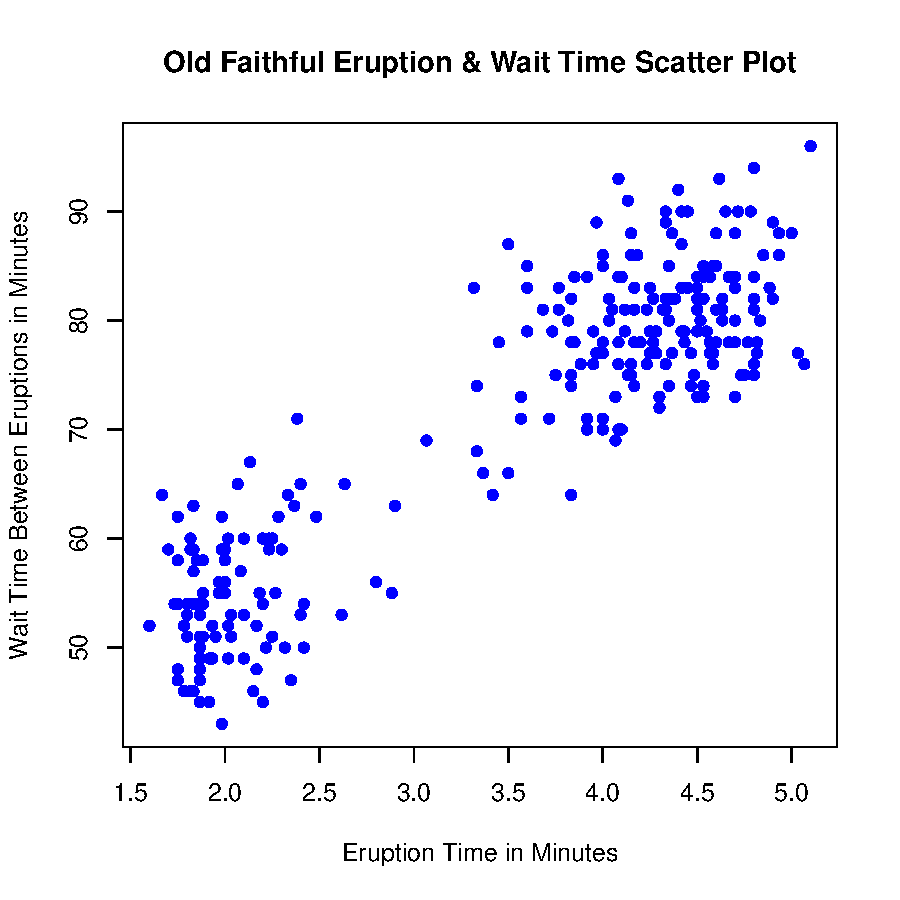
\includegraphics{rnw_example-013}

\underline{Answer:}
\begin{itemize}
\item Added xlab to label the x axis with a descriptive label
\item Added ylab to label the y axis with a descriptive label
\item Added main to give the graph a title to explain what the graph is displaying
\item Added col = blue so that the points would stand out from the background
\item Added pch = 16 so that the points would be filled in circles
\end{itemize}
\underline{References:}
\begin{itemize}
\item https://thomasleeper.com/Rcourse/Tutorials/plotcolors.html
\end{itemize}





\item (5 Points) Provide a careful discussion of the three final graphs, i.e.,
the final histogram for {\it eruptions}, the final histogram for {\it waiting},
and the final scatterplot. It shouldn't matter whether you refer to the ggplot2 or baseR
version as both (hopefully) will show similar information.
Summarize what is shown in each of these three graphs. You need to tell the
reader and verbally describe the most important features.
Use the proper statistical language and refer back to your previously created graphs.

\underline{Answer:}
\begin{itemize}
\item Final Histogram Eruptions: The data in the histogram has a bimodal distribution. With a heavier grouping on the right side of the graph. The eruption times go from 1.625 minutes to 5.125 minutes. The first grouping of eruption times goes from 1.75 minutes to 2.625 minutes. This is the smaller of the two groups in the bimodal distribution. The second grouping of eruption times starts around 3.25 minutes and goes to around 5 minutes. The peak of the first group which is a count of the eruptions that lasted that long is at 24 centered between 1.75 minutes to 1.875 minutes. The second peak reaches a height of 15 and is centered  over 4.5 minutes.

\item Final Histogram Waiting: The final histogram has a bimodal distribution, with a heavier grouping in the right peak.The left peak starts a 43 minutes and ends at 67 minutes. With a high of 9 centered on 54 minutes. The right peak starts at 68 minutes and continues to 96 minutes. With a high of 15 centered over 78 minutes.

\item Final ScatterPlot: The scatterplot shows a positive linear association between eruption time in minutes and the wait time between eruptions.There is some spread to the data so it is not a perfect correlation. For example two plots near the two minute eruption time took anywhere from aound 42.5 minute wait time to a 62.5 minute wait time. The graph also is clearly split into two groups. With a cluster in the 1.75 to 2.5 minute eruption time and the next cluster grouping around the 3.75 to 5 minute wait time.

\end{itemize}





\item (2 Points) Would boxplots be good replacements for the two histograms? 
First create two basic boxplots with a package of your choice.
As always, include your R code and the resulting graphs.
Then answer yes or no. Justify your answer!

\begin{Schunk}
\begin{Sinput}
> b1 <- ggplot(faithful, aes("W", waiting)) +
+   geom_boxplot()
> b2 <- ggplot(faithful, aes("E", eruptions)) +
+   geom_boxplot()
> grid.arrange(b1, b2, ncol = 2)
\end{Sinput}
\end{Schunk}
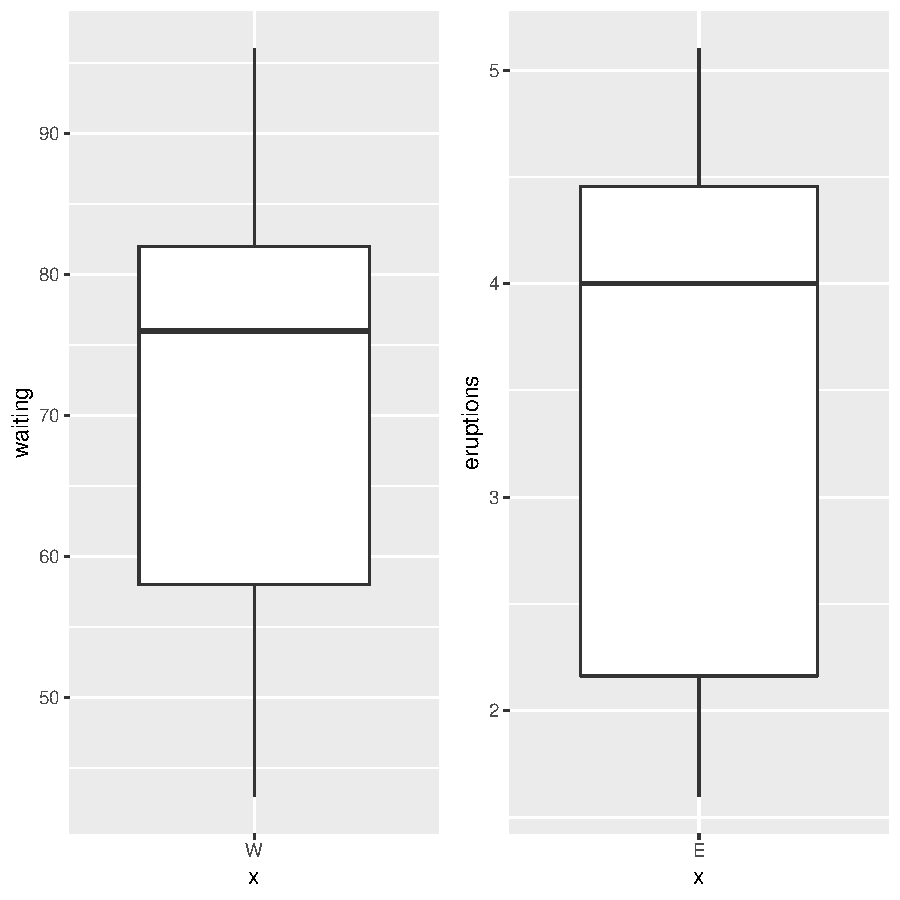
\includegraphics{rnw_example-014}

\underline{Answer:}
\begin{itemize}
\item No, boxplots would not be good replacements for the two histograms. Both histograms show a bimodal distribution for the waiting and eruption data. But in the boxplot you are not able to see this split in the data very well
\end{itemize}





\item (3 Points) Have you ever heard of violin plots? If not, google them!
Find a suitable R package that creates violin plots or see how they can be
created in ggplot2.
Would violin plots be good replacements for the two histograms? 
First create two basic violin plots with a package of your choice.
As always, include your R code and the resulting graphs.
Then answer yes or no. Justify your answer!

\begin{Schunk}
\begin{Sinput}
> par(mfrow = c(1, 2))
> vioplot(faithful$waiting,
+         names = "waiting")
\end{Sinput}
\begin{Soutput}
[1] 43 96
\end{Soutput}
\begin{Sinput}
> vioplot(faithful$eruptions,
+         names = "eruptions")
\end{Sinput}
\begin{Soutput}
[1] 1.6 5.1
\end{Soutput}
\end{Schunk}
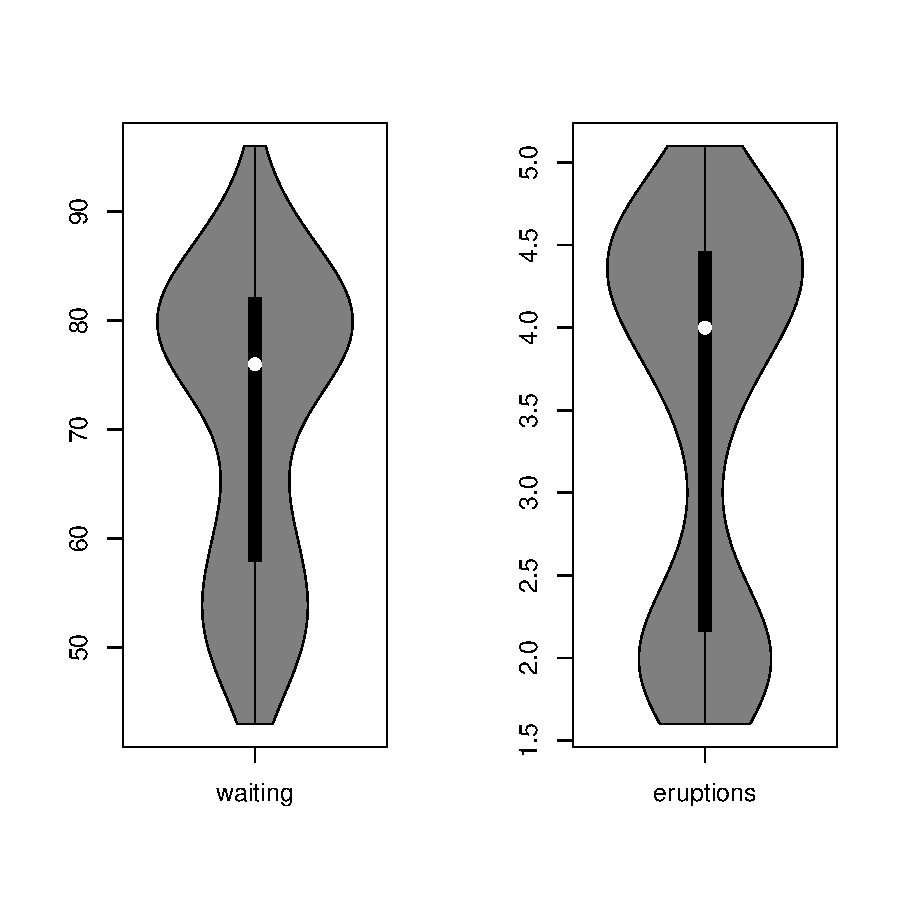
\includegraphics{rnw_example-015}


\underline{Answer:} Yes violion plots would be good replacements for the histograms. They display similar data to a box plot but they allow you to show the distribution of the values so you can see where most of the values are clustering. They also
contain a boxplot so you can get the benefit of both graphs.

\underline{References:} https://www.tutorialgateway.org/r-ggplot2-violin-plot/

\end{enumerate}


\newpage


\item (10 Points)
This question makes use of the {\it geyser} data set from the {\bf MASS} R package, 
an alternative version of the Old Faithful 
data set used in the previous question. The settings used here may or may not be suitable for 
the graphs in the previous question. These graphs may not be perfect and may need some
further adjustments, but those are not required to get full points in this question.


\begin{enumerate}
\item (6 Points) Recreate the graphs (and layout) below using baseR.
Use a ruler to  check that the width and height proportions in your graphs
match the ones I have used. I worked with integer multiples!
Include your R code and the resulting graphs.
Hint: You can create a new line via \verb|\n| without any extra spaces before/after \verb|\n|.

\begin{Schunk}
\begin{Sinput}
> grid <- matrix(c(1, 1, 1, 2, 2, 3, 3, 3, 4, 4), 
+               nrow = 2, ncol = 5, byrow = TRUE)
> layout(grid)
> par(mar = c(4, 3, 4, 2))
> boxplot(geyser$duration,
+         horizontal = TRUE,
+         main = "Old Faithful:\n Duration",
+         ylim = c(0, 6))
> hist(geyser$duration,
+      main = "Old Faithful",
+      xlab = "Duration",
+      ylab = "Count",
+      xlim = c(0, 6))
> boxplot(geyser$waiting,
+         horizontal = TRUE,
+         main = "Old Faithful:\n Waiting",
+         ylim = c(40, 120))
> hist(geyser$waiting,
+      main = "Old Faithful",
+      xlab = "Waiting",
+      ylab = "Count",
+      xlim = c(40, 120),
+      ylim = c(0, 100),
+      breaks = seq(40, 120, by = 10))
\end{Sinput}
\end{Schunk}
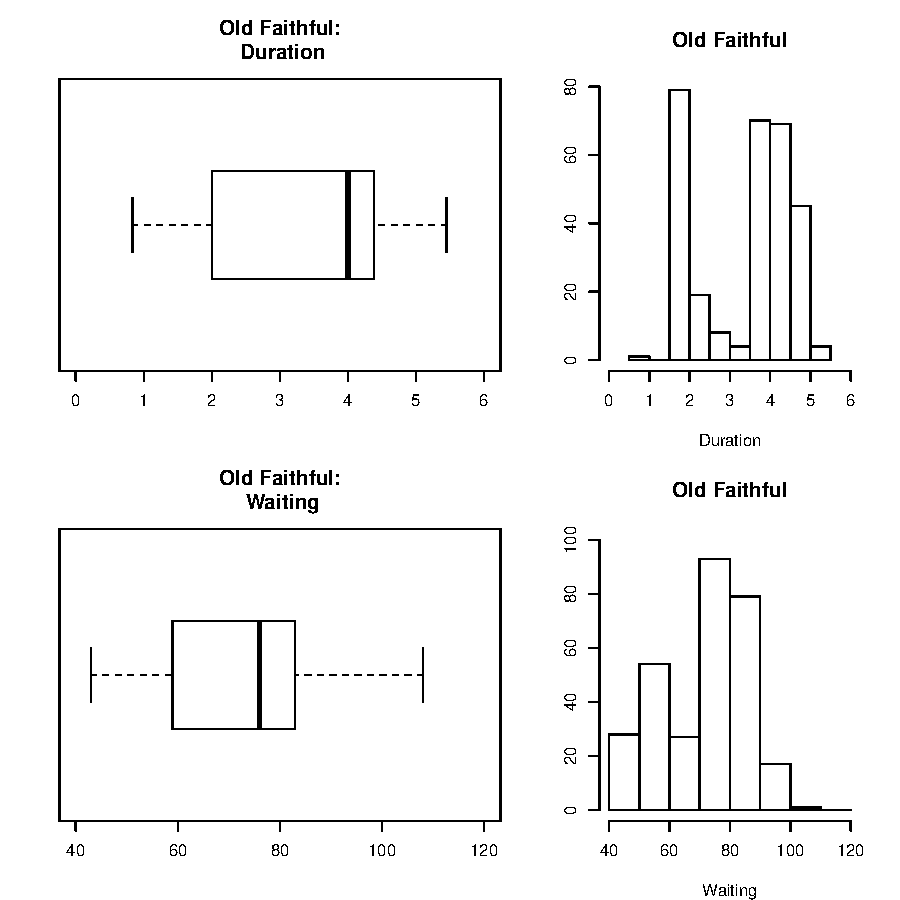
\includegraphics{rnw_example-016}
\underline{Refernces:}
\begin{itemize}
\item https://www.statmethods.net/advgraphs/layout.html
\item https://stackoverflow.com/questions/31319942/change-the-size-of-a-plot-when-plotting-multiple-plots-in-r
\item https://www.youtube.com/watch?v=Z3V4Pbxeahg
\end{itemize}

\begin{figure}[ht]
\centering{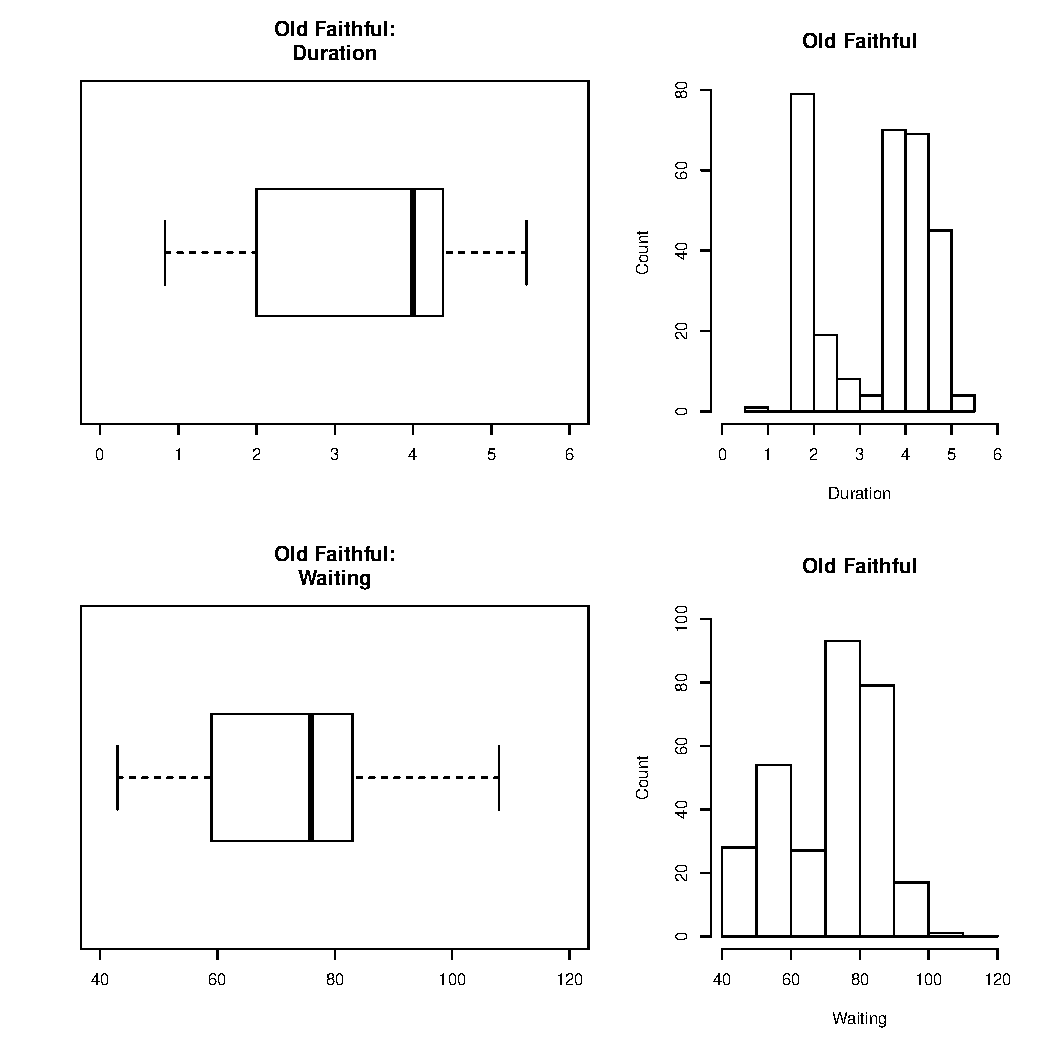
\includegraphics[width=5in]{hw01_q2a.pdf}}
\caption{\label{hw01_q2a}
Graph created with {\it baseR}.
}
\end{figure}



\newpage


\item (2 Points) Recreate the graph below using ggplot2.
Include your R code and the resulting graph.

\begin{Schunk}
\begin{Sinput}
> ggplot(geyser, aes(x=duration, y=waiting)) +
+   geom_point() +
+   xlab("Duration") +
+   ylab("Waiting") +
+   xlim(0, 6) +
+   ylim(40, 120) +
+   ggtitle("Old Faithful Data") +
+   theme(plot.title = element_text(hjust = 0.5))
\end{Sinput}
\end{Schunk}
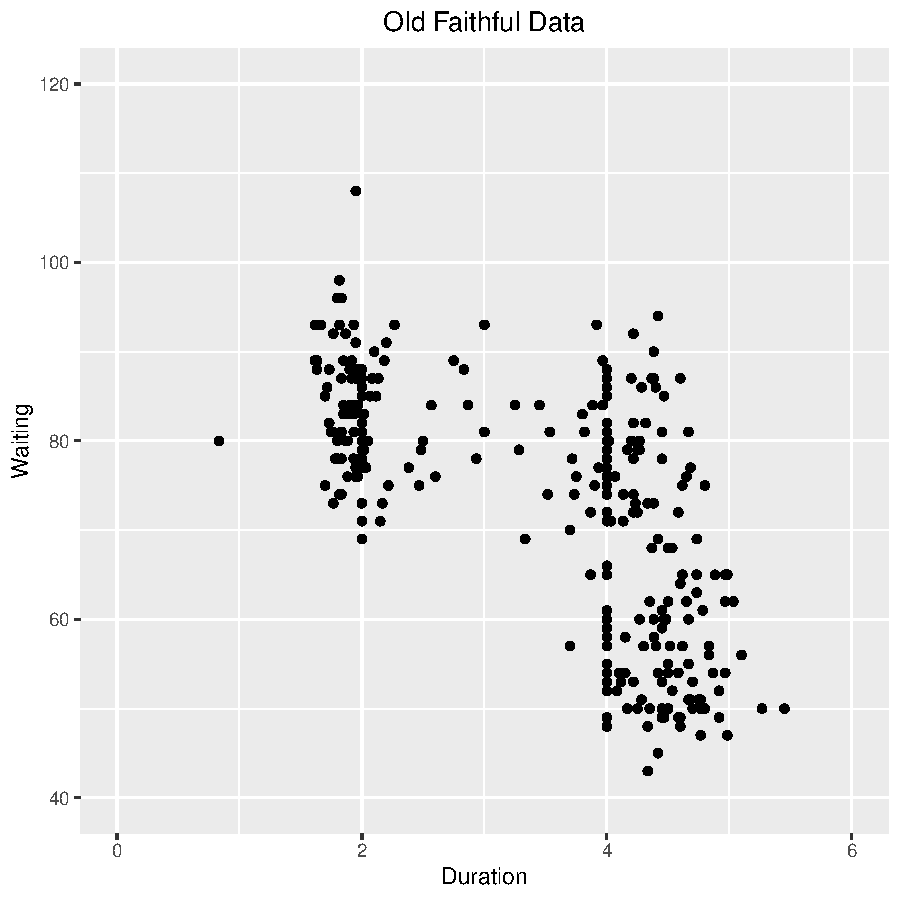
\includegraphics{rnw_example-017}


\begin{figure}[ht]
\centering{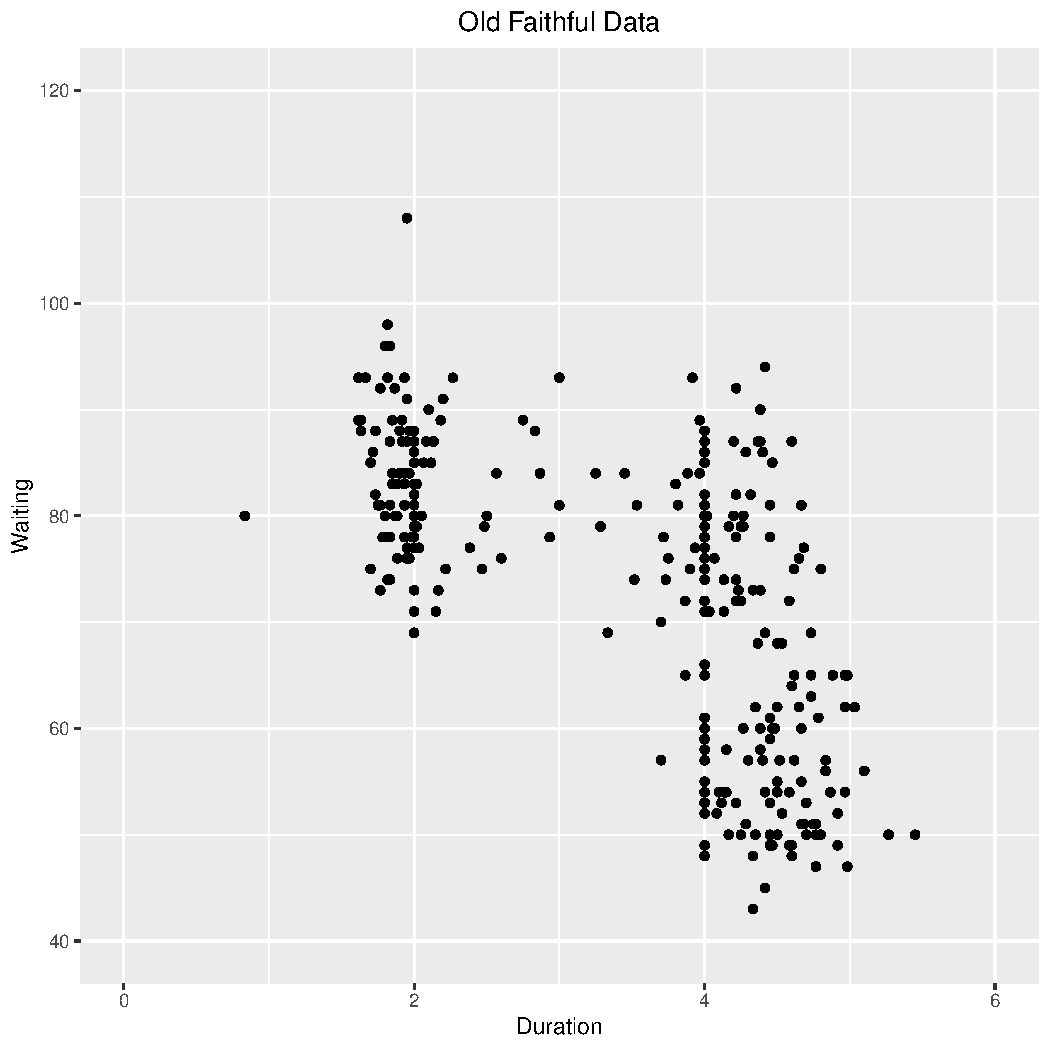
\includegraphics[width=5.0in]{hw01_q2b.pdf}}
\caption{\label{hw01_q2b}
Graph created with {\it ggplot2}.
}
\end{figure}


\newpage


\item (2 Points) Doesn't the scatterplot in (b) above look rather different 
than the scatterplot in Question 1 (j)? Note that the help page for {\it geyser}
states \verb|waiting	 numeric	 Waiting time for this eruption| and \\
\verb|The waiting time was incorrectly described as the time to the next|
\verb|eruption in the original files, and corrected for MASS version 7.3-30.| \\
Use this information to create a basic scatterplot 
for the {\it geyser} data that matches the overall 
appearance in Question 1 (j). 
Include your R code and the resulting graph.
No need to refine this scatterplot.

\begin{Schunk}
\begin{Sinput}
> duration <- geyser$duration[1:298]
> waiting <- geyser$waiting[2:299]
> df <- data.frame(duration, waiting)
> ggplot(df, aes(x = duration, y = waiting )) + 
+          geom_point()
\end{Sinput}
\end{Schunk}
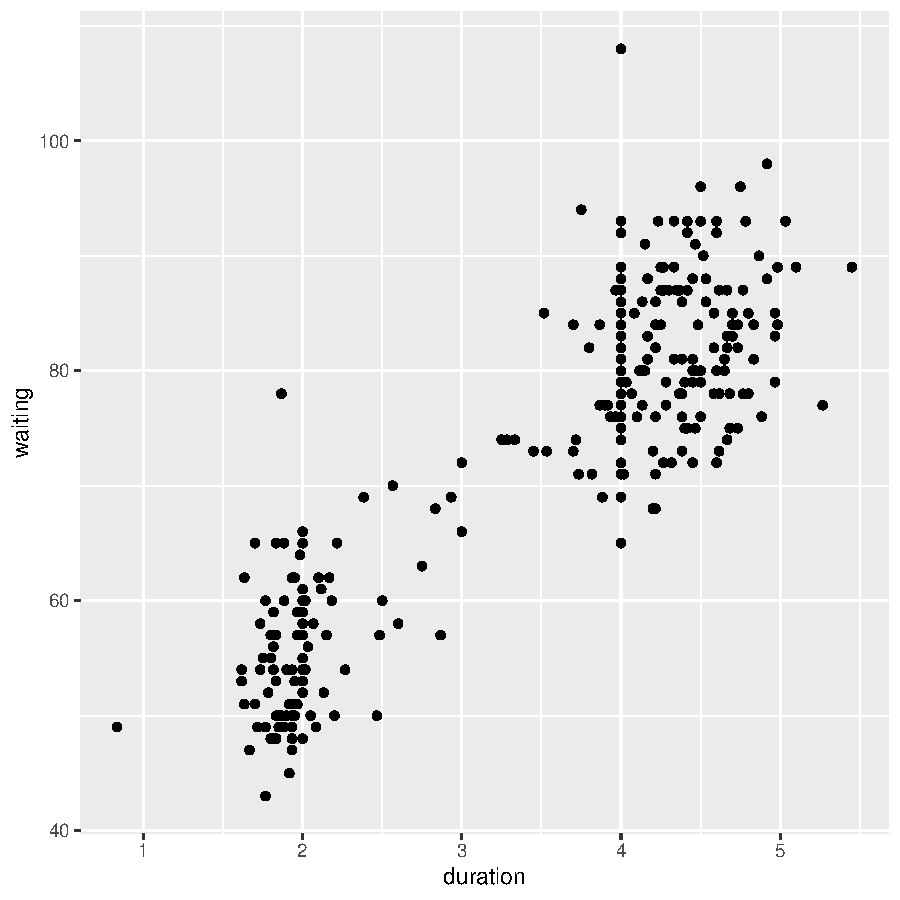
\includegraphics{rnw_example-018}

\underline{Answer:} 
The geyser data appears to have a negative correlation with three clusters where the faithful data has a positive correlation with 2 clusters.


\end{enumerate}

\end{enumerate}


\newpage


\noindent{\Large \bf General Instructions}~\\


\begin{enumerate}
\item Create a single pdf document, using R Markdown, Sweave, or knitr.
%When you take this course at the 6000--level, you have to use \LaTeX\ in
%combination with Sweave or knitr.
You only have to submit this one document to Canvas.

\item Include a title page that contains your name, your A--number, the number of
the assignment, the submission date, and any other relevant information.

\item Start your answers to each main question on a new page (continuing with the next
part of a question on the same page is fine). 
Clearly label each question and question part. Your answer to question (i) should start on page 2!

\item Show your R code and resulting graph(s) for each question part!

\item Before you submit your homework, check that you
follow all recommendations from Google's R Style Guide
(see \url{http://web.stanford.edu/class/cs109l/unrestricted/resources/google-style.html}). 
Moreover, make sure that your R code is consistent, i.e., that you use the same
type of assignments and the same type of quotes throughout your entire homework.

\item Give credit to external sources, such as stackoverflow or help pages. Be specific
and include the full URL where you found the help (or from which help page you got 
the information). Consider R code from such sources as ``legacy code or third--party code'' 
that does not have to be adjusted to Google's R Style (even though it would be nice,
in particular if you only used a brief code segment).

\item {\bf Not following the general instructions outlined above will result in point deductions!}

\item For general questions related to this homework, please
use the corresponding discussion board in Canvas! I will try to
reply as quickly as possible. Moreover, if one of you knows
an answer, please post it. It is fine to refer to web pages
and R commands, but do not provide the exact R command with all required arguments
or which of the suggestions from a stackoverflow web page eventually worked for you! 
This will be the task for each individual student!

\item Submit your single pdf file via Canvas by the submission deadline.
Late submissions will result in point deductions as outlined on the syllabus.

\end{enumerate}


\end{document}

